\documentclass[preprint,12pt,aps,pra,showkeys,amsmath,amssymb,superscriptaddress,floatfix]{revtex4-2}
\usepackage[T1]{fontenc}
\usepackage[utf8]{inputenc}
\usepackage{amsmath,amssymb,amsthm,mathtools,mathrsfs}
\usepackage{microtype,booktabs,enumitem}
\usepackage{xcolor,tikz,etoolbox}
\usepackage[skins,breakable]{tcolorbox}
\usepackage{needspace}
% Keep diagram geometry independent of REVTeX preprint body spacing.
\AtBeginEnvironment{tikzpicture}{\linespread{1}\selectfont}
\usetikzlibrary{arrows.meta,positioning,calc,fit,decorations.pathreplacing}
\usepackage{graphicx}
\usepackage{hyperref}

\definecolor{MMBlue}{RGB}{0,82,155}
\definecolor{MMOrange}{RGB}{200,80,0}
\tikzset{
 mmnode/.style={draw=MMBlue,rounded corners=2pt,fill=MMBlue!4,align=left,execute at begin node={\raggedright},text width=5cm,font=\fontsize{10}{12}\selectfont,inner sep=6pt},
 mmimport/.style={mmnode,draw=black!65,fill=black!4},
 mmcandidate/.style={mmnode,draw=MMOrange,dashed,fill=MMOrange!5},
 mmrejected/.style={mmnode,draw=black,densely dotted,fill=black!8},
 mmproof/.style={->,thick,MMBlue},
 mmflow/.style={->,semithick,black!70},
 mmrepair/.style={->,dashed,thick,MMOrange},
 mmcandidatearrow/.style={->,dashed,semithick,MMOrange},
 mmnote/.style={font=\scriptsize,fill=white,inner sep=2pt,align=center}}

\usepackage[section]{placeins}
\setlength{\emergencystretch}{3em}
\setlist{itemsep=3pt,topsep=4pt}
\newtheorem{theorem}{Theorem}[section]
\newtheorem{proposition}[theorem]{Proposition}
\newtheorem{lemma}[theorem]{Lemma}
\newtheorem{corollary}[theorem]{Corollary}
\theoremstyle{definition}
\newtheorem{definition}[theorem]{Definition}
\newtheorem{example}[theorem]{Example}
\theoremstyle{remark}
\newtheorem{remark}[theorem]{Remark}
% Avoid isolated statement headings and single-line paragraph fragments.
\BeforeBeginEnvironment{theorem}{\Needspace{6\baselineskip}}
\BeforeBeginEnvironment{definition}{\Needspace{5\baselineskip}}
\BeforeBeginEnvironment{proposition}{\Needspace{5\baselineskip}}
\BeforeBeginEnvironment{lemma}{\Needspace{5\baselineskip}}
\BeforeBeginEnvironment{corollary}{\Needspace{5\baselineskip}}
\clubpenalty=5000
\widowpenalty=5000
\newcommand{\R}{\mathbb R}\newcommand{\Z}{\mathbb Z}\newcommand{\N}{\mathbb N}
\newcommand{\Pa}{\operatorname{Pa}}\newcommand{\Desc}{\operatorname{Desc}}
\newcommand{\cl}{\operatorname{cl}}\newcommand{\cost}{\operatorname{cost}}
\newcommand{\status}{\operatorname{status}}
% Faculty cards: a visual rail groups the five faculties within one agent.
% The rail has no arrowhead and does not represent a proof dependency.
\newcommand{\mmfacultybadge}[1]{%
 \node[circle,draw=MMBlue,line width=1pt,fill=white,
 minimum size=7mm,inner sep=0pt,font=\sffamily\small\bfseries,text=MMBlue]
 at ([xshift=15pt,yshift=-15pt]frame.north west) {#1};}
\newcommand{\mmfacultyrail}{%
 \draw[MMBlue!80,line width=1pt]
 ([xshift=15pt,yshift=2pt]frame.north west)--
 ([xshift=15pt,yshift=-2pt]frame.south west);}
\newtcolorbox{mmfacultybox}[2]{enhanced,breakable,
 colback=MMBlue!4,colframe=MMBlue!4,boxrule=0pt,arc=3pt,
 left=39pt,right=9pt,top=4pt,bottom=4pt,
 before skip=2pt,after skip=2pt,
 fontupper=\small\linespread{1.1}\selectfont,
 overlay unbroken={\mmfacultyrail\mmfacultybadge{#1}},
 overlay first={\mmfacultyrail\mmfacultybadge{#1}},
 overlay middle={\mmfacultyrail},overlay last={\mmfacultyrail}}
\newcommand{\mmfaculty}[3]{%
 \begin{mmfacultybox}{#1}{#2}
 {\sffamily\bfseries\color{MMBlue}#2}\par\smallskip #3
 \end{mmfacultybox}}
\newcommand{\agent}[9]{%
 \Needspace{8\baselineskip}
 \subsubsection{#1}
 \noindent\textbf{Object.} #2\par
 \noindent\textbf{Role.} #3\par\smallskip
 \mmfaculty{E}{Ego}{#4}
 \mmfaculty{M}{Memory}{#5}
 \mmfaculty{I}{Intellect}{#6}
 \mmfaculty{S}{Sense}{#7}
 \mmfaculty{A}{Action}{#8}
 \smallskip\noindent #9\par}

\usepackage{longtable,array,calc}
\providecommand{\tightlist}{\setlength{\itemsep}{2pt}\setlength{\parskip}{0pt}}
\makeatletter
\def\frontmatter@abstract@produce{\par\addvspace{\frontmatter@preabstractspace}%
\begingroup\prep@absbox\unvbox\absbox\post@absbox\endgroup
\addvspace{\frontmatter@postabstractspace}}
\makeatother
\newcommand{\field}[2]{\par\smallskip\noindent\textbf{#1.} #2\par}
\setlength{\emergencystretch}{5em}
\AtBeginEnvironment{verbatim}{\small\linespread{1.0}\selectfont}


\hypersetup{colorlinks=true,linkcolor=MMBlue,urlcolor=MMBlue,pdfauthor={Dibakar Sigdel}}

\begin{document}

\title{Linear Convergence of Gradient Descent\\[4pt]\large An End-to-End Meta-Math Walkthrough}

\author{Dibakar Sigdel}

\affiliation{Mindverse Computing LLC, Lynnwood, WA 98087, USA}

\date{October 2026}

\begin{abstract}

Smoothness turns a gradient step into a quantified decrease. Strong
convexity both guarantees an optimum and links the remaining objective
gap to the gradient size. The report presents the target theorem,
declared imports, a dependency graph, five-faculty node contracts, a
continuous proof, a worked example, and a hypothesis-repair audit. It is
an authored mathematical exposition, not a deployed-agent transcript or
a formal proof-assistant certificate.

\end{abstract}\maketitle\linespread{1.12}\selectfont

\noindent\textbf{ON-03 / Optimization and Numerical Analysis / Report v1}

\section{Target and import contract}

\begin{theorem}

Let \(f:\mathbb R^d\to\mathbb R\) be \(C^1\), \(\mu\)-strongly convex,
and have an \(L\)-Lipschitz gradient, with \(0<\mu\le L\). Strong
convexity here means
\(f(y)\ge f(x)+\langle\nabla f(x),y-x\rangle+(\mu/2)\|y-x\|^2\) for
every \(x,y\). Prove there is a unique minimizer \(x_*\) and, for
exact-arithmetic iterates \(x_{k+1}=x_k-\nabla f(x_k)/L\),
\(f(x_k)-f(x_*)\le(1-\mu/L)^k(f(x_0)-f(x_*))\). Also \(x_k\to x_*\).
Interpret the bound at \(k=0\) as equality, including when \(\mu=L\).

\end{theorem}

\subsection{Foundations and permitted imports}

Use the fundamental theorem of calculus along a segment,
Cauchy--Schwarz, and attainment of the minimum of a continuous function
on a compact set. The gradient Lipschitz property is
\(\|\nabla f(x)-\nabla f(y)\|\le L\|x-y\|\). All norms are Euclidean.
The theorem concerns exact iterations and does not certify
rounding-error behavior.

\clearpage\section{Node interaction workflow}

\begin{center}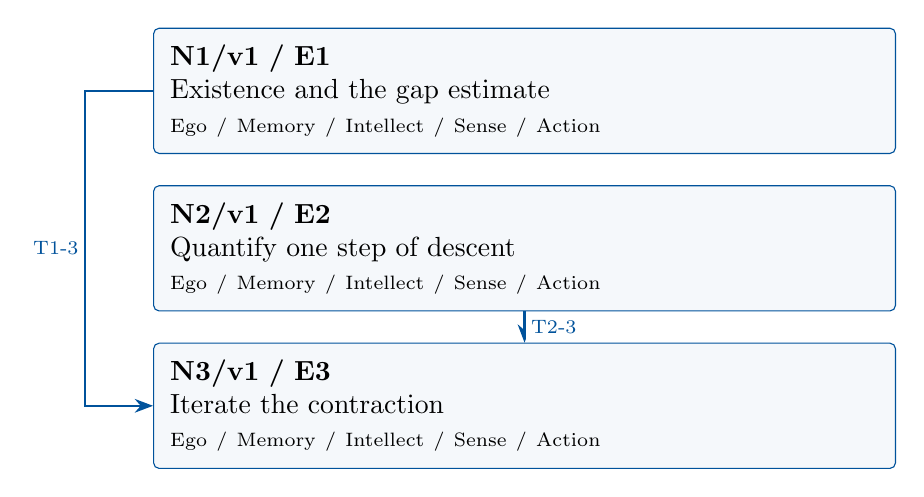
\begin{tikzpicture}[>=Stealth,x=1cm,y=1cm]

\node[mmnode,text width=9cm,minimum height=1.25cm] (N1) at (0,0.0) {\textbf{N1/v1 / E1}\\Existence and the gap estimate\\{\scriptsize Ego / Memory / Intellect / Sense / Action}};

\node[mmnode,text width=9cm,minimum height=1.25cm] (N2) at (0,-2.0) {\textbf{N2/v1 / E2}\\Quantify one step of descent\\{\scriptsize Ego / Memory / Intellect / Sense / Action}};

\node[mmnode,text width=9cm,minimum height=1.25cm] (N3) at (0,-4.0) {\textbf{N3/v1 / E3}\\Iterate the contraction\\{\scriptsize Ego / Memory / Intellect / Sense / Action}};

\draw[mmproof] (N1.west) -- (-5.58,0) -- node[mmnote,left] {T1-3} (-5.58,-4) -- (N3.west);

\draw[mmproof] (N2.south) -- node[mmnote,right] {T2-3} (N3.north);

\end{tikzpicture}\end{center}

Each box is one mathematical agent containing all five faculties. Blue
arrows carry the versioned exports listed below. The layout gives a
reading order; only drawn arrows assert dependencies. Diagnostic repair
is separate from the proof DAG.

\subsection{Versioned evidence-transfer ledger}

\begingroup\small\linespread{1.05}\selectfont

\Needspace{5\baselineskip}\field{T1-3: N1/E1/v1 to N3}{A unique \(x_*\) exists, \(\nabla f(x_*)=0\), and
\(f(x)-f(x_*)\le\|\nabla f(x)\|^2/(2\mu)\).}

\field{Receiving activity}{N3.1}

\field{Compatibility}{E1/v1 and E2/v1 for every iterate. Check: Objective convergence alone is
not automatically convergence of points; the quadratic growth estimate
supplies that bridge.}

\Needspace{5\baselineskip}\field{T2-3: N2/E2/v1 to N3}{\(f(x-\nabla f(x)/L)\le f(x)-\|\nabla f(x)\|^2/(2L)\).}

\field{Receiving activity}{N3.1}

\field{Compatibility}{E1/v1 and E2/v1 for every iterate. Check: Objective convergence alone is
not automatically convergence of points; the quadratic growth estimate
supplies that bridge.}

\endgroup

\clearpage\section{Agent roles and five-faculty activities}\begingroup\small\linespread{1.05}\selectfont\setlist{itemsep=1pt,topsep=2pt}

\subsection{N1/v1: Existence and the gap estimate}

\field{Object and role}{Use a quadratic lower bound for coercivity, then minimize the quadratic
support model. \textbf{Local obligation:} A unique \(x_*\) exists,
\(\nabla f(x_*)=0\), and \(f(x)-f(x_*)\le\|\nabla f(x)\|^2/(2\mu)\).}

\field{Inputs}{Strong convexity with \(\mu>0\).}

\mmfaculty{E}{Ego}{Publish E1/v1 only after establishing this obligation: A unique \(x_*\)
exists, \(\nabla f(x_*)=0\), and
\(f(x)-f(x_*)\le\|\nabla f(x)\|^2/(2\mu)\).}

\mmfaculty{M}{Memory}{Strong convexity with \(\mu>0\). Retain the stated assumptions and
import versions.}

\mmfaculty{I}{Intellect}{Use a quadratic lower bound for coercivity, then minimize the quadratic
support model.}

\mmfaculty{S}{Sense}{The lower bound must grow at infinity; a merely convex function need not
attain its infimum.}

\mmfaculty{A}{Action}{Carry out activities N1.1--N1.2 below, retaining each calculation and
construction as evidence.}

\smallskip\noindent\textbf{Numbered mathematical activities}

\begin{enumerate}[label=N1.\arabic*,leftmargin=3.4em]

\item The strong-convexity inequality at \(x=0\) gives
\(f(y)\ge f(0)+\langle\nabla f(0),y\rangle+(\mu/2)\|y\|^2\to\infty\) as
\(\|y\|\to\infty\). Choose a ball outside which \(f>f(0)\); compact
attainment inside it gives a global minimizer. Differentiability gives
zero gradient there. Strict convexity, which follows from strong
convexity, gives uniqueness (or apply the quadratic lower bound at
either minimizer).

\item For \(g=\nabla f(x)\), strong convexity at \(x\) and \(y=x_*\) gives
\(f(x_*)\ge f(x)+\langle g,x_*-x\rangle+(\mu/2)\|x_*-x\|^2\ge f(x)-\|g\|^2/(2\mu)\)
by completing the square. Rearrangement proves the gap estimate.

\end{enumerate}

\field{Export E1/v1}{A unique \(x_*\) exists, \(\nabla f(x_*)=0\), and
\(f(x)-f(x_*)\le\|\nabla f(x)\|^2/(2\mu)\).}

\field{Acceptance gate}{The lower bound must grow at infinity; a merely convex function need not
attain its infimum.}

\field{Targeted repair}{If the sign of the gradient-gap estimate is reversed, complete the
square explicitly; the resulting bound is a lower bound on gradient size
in terms of the gap. Withhold this export and recheck its descendants
after a versioned correction.}

\clearpage

\subsection{N2/v1: Quantify one step of descent}

\field{Object and role}{Integrate the gradient difference along a segment to derive the descent
lemma. \textbf{Local obligation:}
\(f(x-\nabla f(x)/L)\le f(x)-\|\nabla f(x)\|^2/(2L)\).}

\field{Inputs}{An \(L\)-Lipschitz gradient and \(s=-\nabla f(x)/L\).}

\mmfaculty{E}{Ego}{Publish E2/v1 only after establishing this obligation:
\(f(x-\nabla f(x)/L)\le f(x)-\|\nabla f(x)\|^2/(2L)\).}

\mmfaculty{M}{Memory}{An \(L\)-Lipschitz gradient and \(s=-\nabla f(x)/L\). Retain the stated
assumptions and import versions.}

\mmfaculty{I}{Intellect}{Integrate the gradient difference along a segment to derive the descent
lemma.}

\mmfaculty{S}{Sense}{The factor \(1/2\) comes from integrating \(t\) from zero to one; the
step is exactly \(1/L\).}

\mmfaculty{A}{Action}{Carry out activities N2.1--N2.2 below, retaining each calculation and
construction as evidence.}

\smallskip\noindent\textbf{Numbered mathematical activities}

\begin{enumerate}[label=N2.\arabic*,leftmargin=3.4em]

\item For any vector \(s\), the fundamental theorem gives
\(f(x+s)-f(x)-\langle\nabla f(x),s\rangle=\int_0^1\langle\nabla f(x+ts)-\nabla f(x),s\rangle\,dt\).
Its absolute value is at most \(\int_0^1 Lt\|s\|^2dt=(L/2)\|s\|^2\).

\item Substitute \(s=-\nabla f(x)/L\). The linear term is
\(-\|\nabla f(x)\|^2/L\) and the quadratic term is
\(\|\nabla f(x)\|^2/(2L)\), giving the claimed decrease.

\end{enumerate}

\field{Export E2/v1}{\(f(x-\nabla f(x)/L)\le f(x)-\|\nabla f(x)\|^2/(2L)\).}

\field{Acceptance gate}{The factor \(1/2\) comes from integrating \(t\) from zero to one; the
step is exactly \(1/L\).}

\field{Targeted repair}{If arbitrary positive step sizes are declared descending, retain the
smoothness quadratic term and verify its coefficient before choosing a
step. Withhold this export and recheck its descendants after a versioned
correction.}

\clearpage

\subsection{N3/v1: Iterate the contraction}

\field{Object and role}{Combine the gap-gradient inequality with one-step descent, then control
distance by strong convexity at the minimizer. \textbf{Local
obligation:} The stated geometric objective bound holds and
\(\|x_k-x_*\|^2\le2(f(x_k)-f(x_*))/\mu\to0\).}

\field{Inputs}{E1/v1 and E2/v1 for every iterate. Incoming proof exports: E1/v1 at
N3.1, E2/v1 at N3.1.}

\mmfaculty{E}{Ego}{Publish E3/v1 only after establishing this obligation: The stated
geometric objective bound holds and
\(\|x_k-x_*\|^2\le2(f(x_k)-f(x_*))/\mu\to0\).}

\mmfaculty{M}{Memory}{E1/v1 and E2/v1 for every iterate. Incoming proof exports: E1/v1 at
N3.1, E2/v1 at N3.1. Retain the stated assumptions and import versions.}

\mmfaculty{I}{Intellect}{Combine the gap-gradient inequality with one-step descent, then control
distance by strong convexity at the minimizer.}

\mmfaculty{S}{Sense}{Objective convergence alone is not automatically convergence of points;
the quadratic growth estimate supplies that bridge.}

\mmfaculty{A}{Action}{Carry out activities N3.1--N3.2 below, retaining each calculation and
construction as evidence.}

\smallskip\noindent\textbf{Numbered mathematical activities}

\begin{enumerate}[label=N3.\arabic*,leftmargin=3.4em]

\item Put \(\Delta_k=f(x_k)-f(x_*)\ge0\). E2 and E1 give
\(\Delta_{k+1}\le\Delta_k-\|\nabla f(x_k)\|^2/(2L)\le(1-\mu/L)\Delta_k\).
Induction gives the geometric bound. If \(\mu=L\), the first step has
gap zero and all later iterates are the minimizer.

\item Strong convexity at \(x_*\), where the gradient is zero, gives
\(\Delta_k\ge(\mu/2)\|x_k-x_*\|^2\). The objective bound therefore
implies convergence of the iterates themselves. This completes the
existence, rate, and convergence claims.

\end{enumerate}

\field{Export E3/v1}{The stated geometric objective bound holds and
\(\|x_k-x_*\|^2\le2(f(x_k)-f(x_*))/\mu\to0\).}

\field{Acceptance gate}{Objective convergence alone is not automatically convergence of points;
the quadratic growth estimate supplies that bridge.}

\field{Targeted repair}{If point convergence is inferred solely from function values, insert the
positive quadratic growth bound with its factor \(\mu/2\). Withhold this
export and recheck its descendants after a versioned correction.}

\endgroup\clearpage\section{Continuous mathematical proof}\label{sec:proof}

\subsection{N1 --- Existence and the gap
estimate}\label{n1-existence-and-the-gap-estimate}

\begin{enumerate}
\def\labelenumi{\arabic{enumi}.}
\item
  \textbf{N1.1.} The strong-convexity inequality at \(x=0\) gives
  \(f(y)\ge f(0)+\langle\nabla f(0),y\rangle+(\mu/2)\|y\|^2\to\infty\)
  as \(\|y\|\to\infty\). Choose a ball outside which \(f>f(0)\); compact
  attainment inside it gives a global minimizer. Differentiability gives
  zero gradient there. Strict convexity, which follows from strong
  convexity, gives uniqueness (or apply the quadratic lower bound at
  either minimizer).
\item
  \textbf{N1.2.} For \(g=\nabla f(x)\), strong convexity at \(x\) and
  \(y=x_*\) gives
  \(f(x_*)\ge f(x)+\langle g,x_*-x\rangle+(\mu/2)\|x_*-x\|^2\ge f(x)-\|g\|^2/(2\mu)\)
  by completing the square. Rearrangement proves the gap estimate.
\end{enumerate}

\subsection{N2 --- Quantify one step of
descent}\label{n2-quantify-one-step-of-descent}

\begin{enumerate}
\def\labelenumi{\arabic{enumi}.}
\item
  \textbf{N2.1.} For any vector \(s\), the fundamental theorem gives
  \(f(x+s)-f(x)-\langle\nabla f(x),s\rangle=\int_0^1\langle\nabla f(x+ts)-\nabla f(x),s\rangle\,dt\).
  Its absolute value is at most \(\int_0^1 Lt\|s\|^2dt=(L/2)\|s\|^2\).
\item
  \textbf{N2.2.} Substitute \(s=-\nabla f(x)/L\). The linear term is
  \(-\|\nabla f(x)\|^2/L\) and the quadratic term is
  \(\|\nabla f(x)\|^2/(2L)\), giving the claimed decrease.
\end{enumerate}

\subsection{N3 --- Iterate the
contraction}\label{n3-iterate-the-contraction}

\begin{enumerate}
\def\labelenumi{\arabic{enumi}.}
\item
  \textbf{N3.1.} Put \(\Delta_k=f(x_k)-f(x_*)\ge0\). E2 and E1 give
  \(\Delta_{k+1}\le\Delta_k-\|\nabla f(x_k)\|^2/(2L)\le(1-\mu/L)\Delta_k\).
  Induction gives the geometric bound. If \(\mu=L\), the first step has
  gap zero and all later iterates are the minimizer.
\item
  \textbf{N3.2.} Strong convexity at \(x_*\), where the gradient is
  zero, gives \(\Delta_k\ge(\mu/2)\|x_k-x_*\|^2\). The objective bound
  therefore implies convergence of the iterates themselves. This
  completes the existence, rate, and convergence claims.
\end{enumerate}

\hfill$\square$

\section{Worked orchestration}

For \(f(x,y)=(x^2+4y^2)/2\), take \(\mu=1\), \(L=4\). The iteration
sends \((x,y)\) to \((3x/4,0)\). From \((1,1)\) the first objective
drops from \(5/2\) to \(9/32\), below the certified upper bound
\((3/4)(5/2)=15/8\). Later the actual remaining gap shrinks by \(9/16\)
per step, so the theorem's \(3/4\) factor is conservative.

\subsection{Boundary and hypothesis audit}

An arbitrary large step fails even for \(f(x)=x^2/2\). With step size
\(3\) the iteration is \(x_{k+1}=-2x_k\), and the objective grows by a
factor of four unless \(x_0=0\). The prescribed step and smoothness
bound cannot be discarded.

\section{Illustrative failure and repair}

The following is an authored diagnostic scenario. Changed assumptions
define a new contract; they do not retroactively prove the original
statement.

\subsection{Rejected argument, diagnosis, and correction}
\textbf{Rejected N3 argument:} decreasing objective values guarantee
convergence to the unique optimum with a geometric rate. Monotone
numbers alone provide neither conclusion. \textbf{Diagnosis:} Intellect
omitted the quantitative gradient-gap bridge. \textbf{Repair:} use E1 to
obtain the actual contraction factor and the strong-convexity distance
estimate. This completes the original theorem under its existing
assumptions; recheck both objective and point convergence.

\subsection{Publication and reuse}
The corrected export retains its explicit assumptions. A hypothetical
revision receives a new version, and each consuming activity is
rechecked; this scenario is not a recorded runtime event. \textbf{Next
direction:} Investigate accelerated methods or inexact gradients with
newly stated error bounds; do not transfer this exact-arithmetic rate
unchanged.

\par\medskip\begingroup\small\linespread{1.0}\selectfont\noindent\textbf{Provenance.} This authored proof is complete relative to its declared imports. Reuse
each export with its assumptions, proof, and version. The original
Markdown remains available for comparison.
\par\endgroup

\par\smallskip\begingroup\small\linespread{1.0}\selectfont\noindent\textbf{Further reading.} \href{https://web.stanford.edu/~boyd/cvxbook/}{Boyd and Vandenberghe,
Convex Optimization} for convexity, optimality, and descent;
\href{https://www.math.umd.edu/~mariakc/Spring2020Class.html}{University
of Maryland, Scientific Computing I} for the numerical-analysis setting.
The estimates used here are derived explicitly in §4.\par\endgroup

\end{document}
